\documentclass[landscape,letterpaper]{article}
\usepackage[left=5pt,top=5pt,right=20pt]{geometry}
\usepackage{tikz}
\begin{document}

\begin{center}
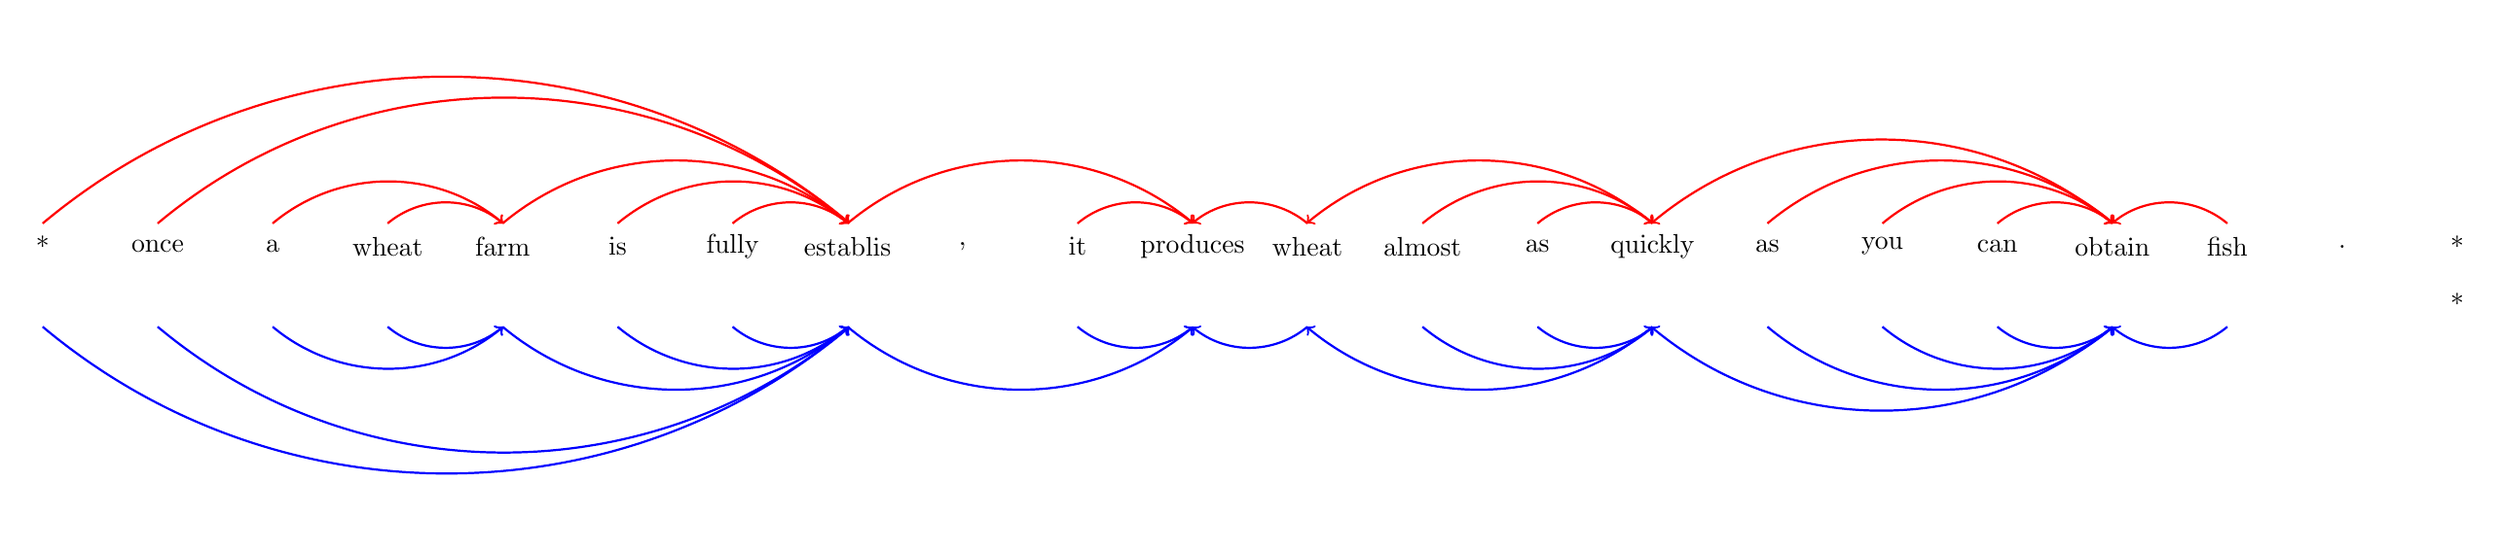
\begin{tikzpicture}[scale=1.5]
\draw(0,0) node {*};
\draw(0,-0.5) node {};
\draw(1,0) node {once};
\draw(1,-0.5) node {};
\draw(2,0) node {a};
\draw(2,-0.5) node {};
\draw(3,0) node {wheat};
\draw(3,-0.5) node {};
\draw(4,0) node {farm};
\draw(4,-0.5) node {};
\draw(5,0) node {is};
\draw(5,-0.5) node {};
\draw(6,0) node {fully};
\draw(6,-0.5) node {};
\draw(7,0) node {establis};
\draw(7,-0.5) node {};
\draw(8,0) node {,};
\draw(8,-0.5) node {};
\draw(9,0) node {it};
\draw(9,-0.5) node {};
\draw(10,0) node {produces};
\draw(10,-0.5) node {};
\draw(11,0) node {wheat};
\draw(11,-0.5) node {};
\draw(12,0) node {almost};
\draw(12,-0.5) node {};
\draw(13,0) node {as};
\draw(13,-0.5) node {};
\draw(14,0) node {quickly};
\draw(14,-0.5) node {};
\draw(15,0) node {as};
\draw(15,-0.5) node {};
\draw(16,0) node {you};
\draw(16,-0.5) node {};
\draw(17,0) node {can};
\draw(17,-0.5) node {};
\draw(18,0) node {obtain};
\draw(18,-0.5) node {};
\draw(19,0) node {fish};
\draw(19,-0.5) node {};
\draw(20,0) node {.};
\draw(20,-0.5) node {};
\draw(21,0) node {*};
\draw(21,-0.5) node {*};
\draw[thick,red,->] (0,0.2) arc(130:50:5.46);
\draw[thick,red,->] (1,0.2) arc(130:50:4.68);
\draw[thick,red,->] (2,0.2) arc(130:50:1.56);
\draw[thick,red,->] (3,0.2) arc(130:50:0.78);
\draw[thick,red,->] (4,0.2) arc(130:50:2.34);
\draw[thick,red,->] (5,0.2) arc(130:50:1.56);
\draw[thick,red,->] (6,0.2) arc(130:50:0.78);
\draw[thick,red,->] (7,0.2) arc(130:50:2.34);
\draw[thick,red,->] (9,0.2) arc(130:50:0.78);
\draw[thick,red,->] (11,0.2) arc(50:130:0.78);
\draw[thick,red,->] (12,0.2) arc(130:50:1.56);
\draw[thick,red,->] (13,0.2) arc(130:50:0.78);
\draw[thick,red,->] (14,0.2) arc(50:130:2.34);
\draw[thick,red,->] (15,0.2) arc(130:50:2.34);
\draw[thick,red,->] (16,0.2) arc(130:50:1.56);
\draw[thick,red,->] (17,0.2) arc(130:50:0.78);
\draw[thick,red,->] (18,0.2) arc(50:130:3.12);
\draw[thick,red,->] (19,0.2) arc(50:130:0.78);
\draw[thick,blue,->] (0,-0.7) arc(50:130:-5.46);
\draw[thick,blue,->] (1,-0.7) arc(50:130:-4.68);
\draw[thick,blue,->] (2,-0.7) arc(50:130:-1.56);
\draw[thick,blue,->] (3,-0.7) arc(50:130:-0.78);
\draw[thick,blue,->] (4,-0.7) arc(50:130:-2.34);
\draw[thick,blue,->] (5,-0.7) arc(50:130:-1.56);
\draw[thick,blue,->] (6,-0.7) arc(50:130:-0.78);
\draw[thick,blue,->] (7,-0.7) arc(50:130:-2.34);
\draw[thick,blue,->] (9,-0.7) arc(50:130:-0.78);
\draw[thick,blue,->] (11,-0.7) arc(130:50:-0.78);
\draw[thick,blue,->] (12,-0.7) arc(50:130:-1.56);
\draw[thick,blue,->] (13,-0.7) arc(50:130:-0.78);
\draw[thick,blue,->] (14,-0.7) arc(130:50:-2.34);
\draw[thick,blue,->] (15,-0.7) arc(50:130:-2.34);
\draw[thick,blue,->] (16,-0.7) arc(50:130:-1.56);
\draw[thick,blue,->] (17,-0.7) arc(50:130:-0.78);
\draw[thick,blue,->] (18,-0.7) arc(130:50:-3.12);
\draw[thick,blue,->] (19,-0.7) arc(130:50:-0.78);
\end{tikzpicture}
\end{center}

\end{document}